\documentclass{article}
\usepackage{tikz}
\usetikzlibrary{3d, perspective}
\begin{document}

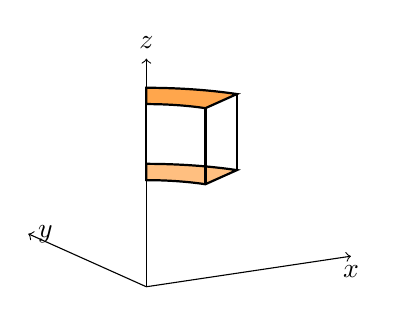
\begin{tikzpicture}[3d view, perspective={p = {(5, 4, 3)}, q = {(0,0,0)}}]
    % Axes
    \draw[->] (0,0,0) -- (3,0,0) node[below] {$x$};
    \draw[->] (0,0,0) -- (0,3,0) node[right] {$y$};
    \draw[->] (0,0,0) -- (0,0,3) node[above] {$z$};

    % Cylindrical Element
    \def\r{1.5}
    \def\dr{0.8}
    \def\th{30}
    \def\dth{30}
    \def\z{1}
    \def\dz{1}
    
    % Base at z
    \begin{scope}[canvas is xy plane at z=\z]
        \draw[thick, fill=orange!50] 
            (\th:\r) arc (\th:\th+\dth:\r) -- 
            (\th+\dth:\r+\dr) arc (\th+\dth:\th:\r+\dr) -- cycle;
    \end{scope}
    
    % Top at z+dz
    \begin{scope}[canvas is xy plane at z=\z+\dz]
        \draw[thick, fill=orange!70] 
            (\th:\r) arc (\th:\th+\dth:\r) -- 
            (\th+\dth:\r+\dr) arc (\th+\dth:\th:\r+\dr) -- cycle;
    \end{scope}

    % Vertical lines connecting them
    \draw[thick] (\th:\r)++(0,0,\z) -- ++(0,0,\dz);
    \draw[thick] (\th+\dth:\r)++(0,0,\z) -- ++(0,0,\dz);
    \draw[thick] (\th:\r+\dr)++(0,0,\z) -- ++(0,0,\dz);
    \draw[thick] (\th+\dth:\r+\dr)++(0,0,\z) -- ++(0,0,\dz);

\end{tikzpicture}

\end{document}
